\chapter{MAC-IO: Self-Supervised Inertial Odometry for New Embodiments} \label{chapter:macio}
\fancyhead[LO]{\makebox[\textwidth][r]{Chapter 6. MAC-IO}}

\begin{framed}
    \centering
    \textbf{Research Question 4 (Self-Supervised Inertial Odometry for Arbitrary Embodiments)} \\
    \textit{How can a learning-based inertial odometry network adapt to a new robot embodiment using only unlabeled IMU data, without motion capture, GNSS, or other externally supplied ground-truth trajectories?} \\[0.3em]
    \emph{Addressed by} \textbf{MAC-IO}.
\end{framed}

\begin{figure}[!htbp]
\centering
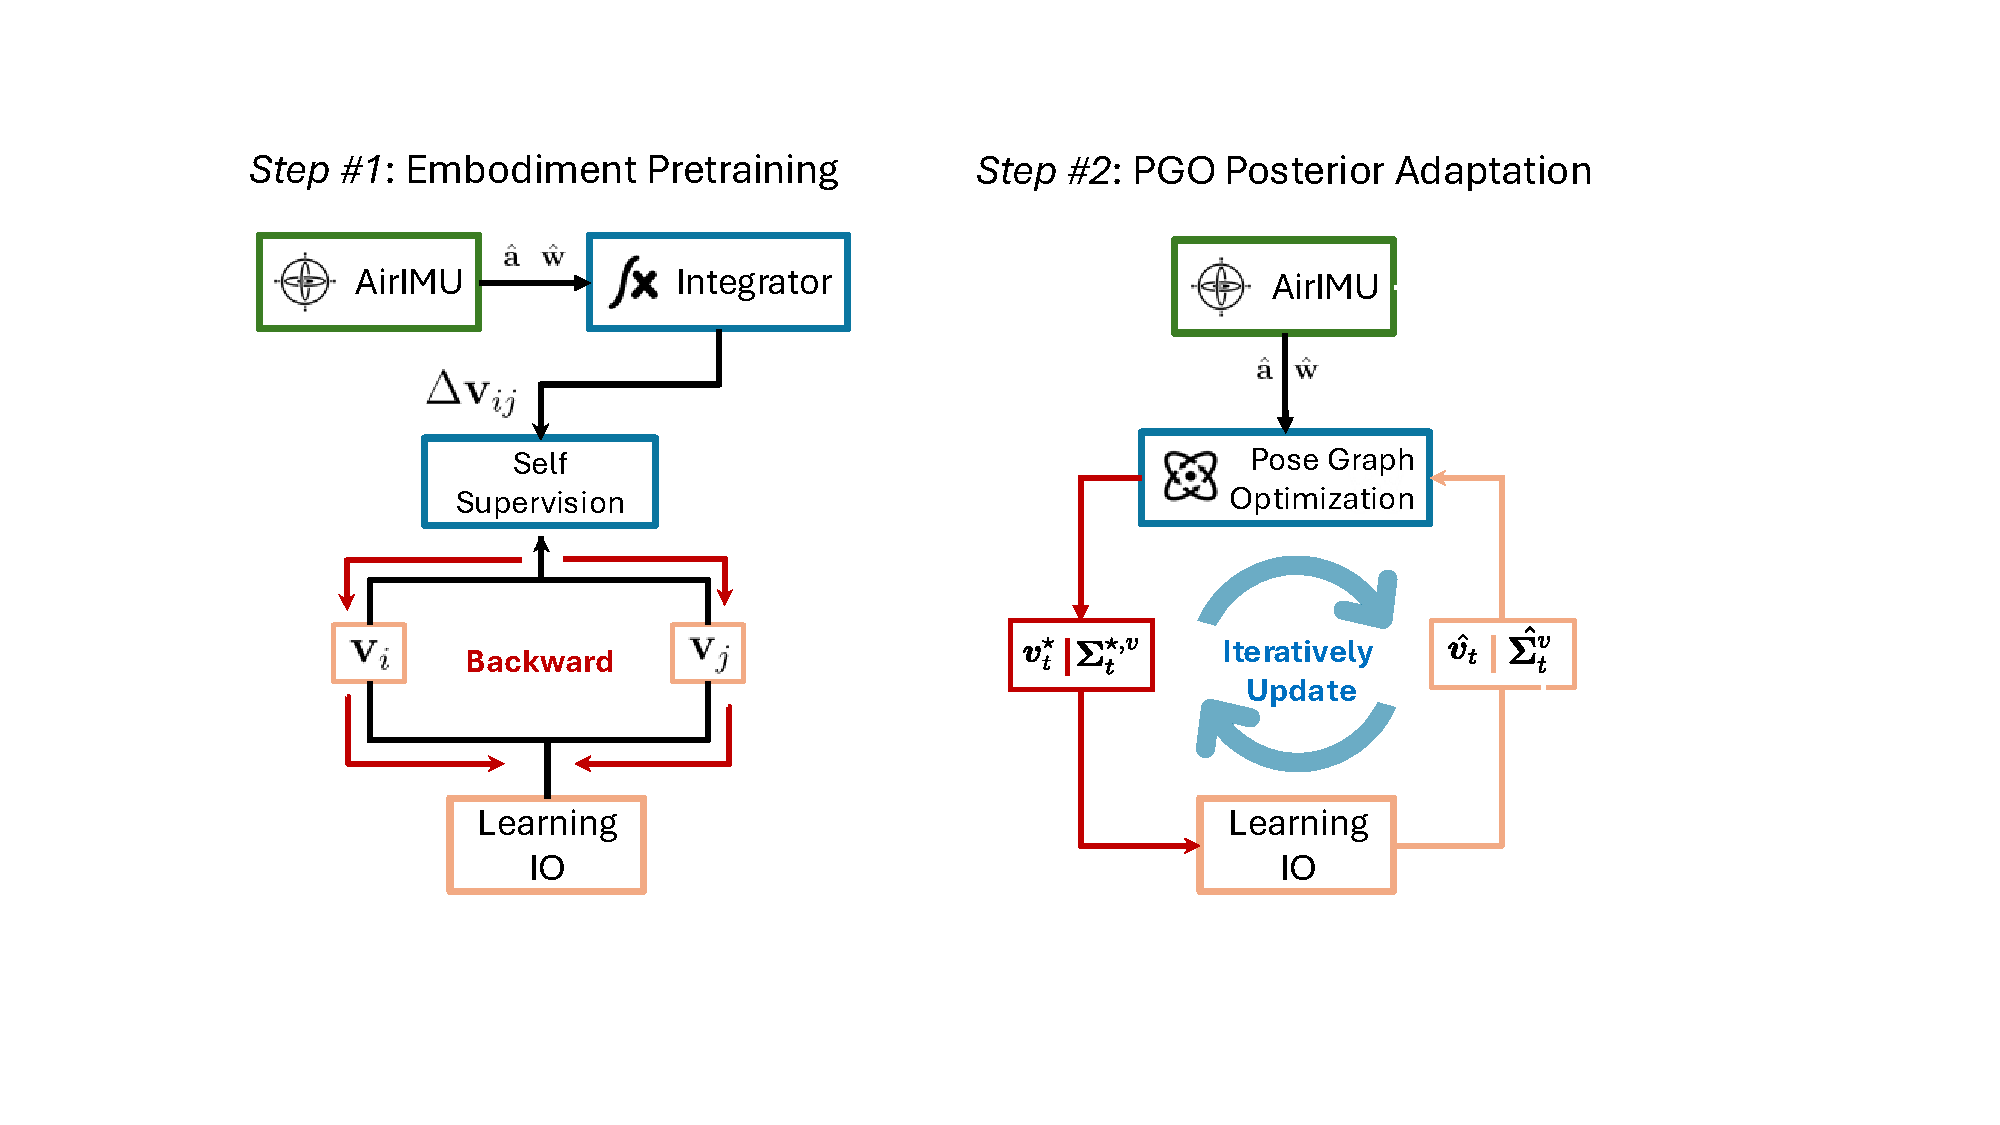
\includegraphics[width=0.95\linewidth]{tex/ch6_macio/figs/overview.pdf}
\caption[MAC-IO learns inertial odometry for a new embodiment from unlabeled IMU.]{\textbf{MAC-IO learns inertial odometry for a new embodiment from unlabeled IMU in two steps.}
\textbf{Step~1} (Embodiment Pretraining) trains the motion network from scratch with self-supervision from a frozen IMU preintegration teacher (instantiated with AirIMU in our implementation), using a Mahalanobis loss on body-frame velocity increments.
\textbf{Step~2} (PGO Posterior Adaptation) iteratively distills the velocity and covariance posterior of a sliding-window pose graph that fuses the same preintegration teacher with the pretrained network's velocity factors, and uses the posterior as dense pseudo-labels for fine-tuning.}
\label{fig:macio:overview}
\end{figure}

\section{Introduction}
\label{sec:macio:intro}

Reliable odometry remains difficult when cameras, LiDAR, or GNSS become unavailable.
Inertial measurement units (IMUs) are cheap, compact, and robust to visual degradation, but IMU-only odometry suffers from noise and bias that accumulate into drift.
Learning-based inertial odometry (IO) reduces this drift by learning motion priors from supervised pose or velocity labels~\cite{chen2018ionet, yan2018ridi, herath2020ronin, liu2020tlio, qiu2025airio}.
The central deployment challenge is that these learned priors transfer poorly across both embodiment classes and embodiment variants.
Across classes, contact-driven legged motion and thrust-driven flight obey different motion regularities.
Within a class, two humanoids can still differ in height, mass, gait behavior, and IMU mounting, which changes how inertial measurements relate to body velocity.
As a result, a learned IO model trained on one embodiment often requires new supervision before it works reliably on another.

In practice, scaling learned IO across embodiments is limited by the need for labeled data on each new platform.
Obtaining those labels is often the hardest part of deploying learned IO.
Motion capture, RTK, LiDAR, and visual-inertial SLAM each require favorable infrastructure, signals, or sensing conditions.
These requirements become harder to satisfy for agile drones, legged robots, and fielded humanoids because each new mounting, payload, motion regime, or deployment environment may require another labeled collection.
The relevant environments can include indoor laboratories, outdoor open areas, cluttered buildings, uneven terrain, and visually degraded scenes, many of which are hard to control or instrument.

This label bottleneck is costly for individual deployments and also limits a foundation-model path for IO.
A broadly deployable IO model would need coverage over many bodies, mountings, payloads, and motion regimes, but supervised training would require pose or velocity labels for each of them.
In contrast, unlabeled IMU streams are easy to collect from deployed systems.
This gap motivates our main question: \textit{Can the IMU perception model learn an embodiment-specific motion prior from unlabeled IMU alone?}

Although motion priors are embodiment-specific, the inertial integration model provides a universal physical structure shared by all IMU platforms.
The standard IMU kinematic integration equations constrain how angular velocity and specific force accumulate into changes in orientation, velocity, and position.
Classical preintegration uses this structure to summarize high-rate IMU measurements as relative-motion factors for state estimation~\cite{forster2015imu}.
AirIMU (Chapter~\ref{chapter:airimu}) further learns to correct preintegration and estimate its uncertainty, making this physical signal more suitable as a data-driven teacher~\cite{qiu2023airimu}.
For unlabeled learning, the same structure can provide pseudo-supervision that depends only on the IMU stream, not on external pose or velocity labels.
Our key idea is to maximally leverage this universal integration structure to create self-supervision from unlabeled IMU, while still letting the learned motion prior specialize to the target embodiment.

We propose \textbf{MAC-IO}, a self-supervised pretrain-then-adapt pipeline for learning IO on a new embodiment from unlabeled IMU.
The first step, embodiment pretraining, starts from scratch and matches network-predicted velocity increments to IMU preintegration increments with a Mahalanobis loss.
This teacher can be any frozen IMU integration module that provides velocity increments and uncertainty; in our implementation, we use AirIMU as an optional correction and uncertainty model to improve the quality of the preintegration teacher.
This local supervision is informative but incomplete: velocity increments teach how motion changes, but they are invariant to constant velocity offsets and do not determine the full velocity estimate.
The second step, PGO posterior adaptation, adds the missing sequence-level constraint.
A sliding-window pose graph fuses IMU preintegration factors with pretrained network velocity factors, approximates the local posterior around the optimized graph, and distills posterior velocity values and covariance back into the same network.

MAC-IO separates the roles of local and sequence-level self-supervision.
Embodiment pretraining learns how recent IMU patterns explain short-horizon velocity changes.
PGO posterior adaptation supplies the missing sequence-level constraint on velocity value and uncertainty.
The core protocol is fully self-supervised: the motion network starts from random initialization, uses no embodiment labels, and trains only from unlabeled IMU with model-derived targets.
On TLIO, this raw-IMU protocol reaches the AVE shown in \fref{fig:macio:setup1_ssl_results} after Step~2, becoming competitive with supervised pretrained references without using embodiment labels.
We also study a separate pretrained-model setting, where the same PGO posterior adaptation improves a supervised pretrained IO model by the multiplicative AVE reductions reported in \tref{tab:macio:setup2_summary} (up to $2.6\times$ in network AVE on TLIO, and $3.1\times$ when followed by PGO at inference).

In summary, this chapter makes the following contributions:
\begin{enumerate}
    \item We formulate embodiment adaptation for learned inertial odometry as a self-supervised learning problem from unlabeled IMU, motivated by the high cost of collecting pose or velocity labels across robots, mountings, and environments.
    \item We introduce MAC-IO, a pretrain-then-adapt framework that leverages universal inertial integration to create pseudo-supervision from unlabeled IMU: velocity-increment pretraining learns local embodiment-specific motion changes, and PGO posterior adaptation distills sequence-level velocity and uncertainty into the network.
    \item We evaluate MAC-IO under two protocols: self-supervised training from scratch and self-supervised adaptation of a supervised pretrained model. On TLIO, self-supervised adaptation reaches centimeter-level accuracy at $\sim$0.03~m/s AVE on unlabeled IMU, improving the pretrained reference by $2.6\times$ in network AVE and by $3.1\times$ when combined with PGO at inference.
\end{enumerate}

\section{Related Work}
\label{sec:macio:relatedwork}

\textbf{Learning-based inertial odometry.}
Early neural IO systems showed that IMU windows contain motion cues beyond what classical dead reckoning can recover from noisy integration alone.
IONet learns inertial odometry from raw IMU sequences~\cite{chen2018ionet}, RIDI exploits pedestrian motion constraints~\cite{yan2018ridi}, RoNIN scales neural inertial navigation to in-the-wild phone data~\cite{herath2020ronin}, and TLIO tightly couples learned velocity with filtering~\cite{liu2020tlio}.
Recent systems extend learned IO to drones and other robots by changing the representation or dynamics model~\cite{cioffi2023learned, qiu2025airio}.
AirIO improves learned aerial inertial odometry by using a body-frame representation that enhances IMU feature observability and by training with supervised trajectory labels~\cite{qiu2025airio}.
These methods improve accuracy when labeled training data match the deployment embodiment.
They still rely on supervised velocity or pose labels to learn the motion prior that maps inertial patterns to body motion.
MAC-IO targets the complementary problem: it learns or adapts this embodiment-specific motion prior from unlabeled IMU on the new embodiment.

\textbf{Uncertainty-aware inertial estimation.}
Classical preintegration provides a compact factor for fusing high-rate IMU measurements in optimization or filtering~\cite{forster2015imu}.
Learning-based inertial models can estimate bias, correction terms, or uncertainty that make inertial factors more robust inside downstream estimators~\cite{buchanan2022deep, qiu2023airimu}.
Deep IMU Bias infers IMU bias terms for robust visual-inertial factor graphs, while AirIMU learns IMU corrections and covariance propagation for inertial odometry.
MAC-IO uses this metrics-aware covariance as a Mahalanobis metric for velocity-increment supervision, not only as a weight inside a state estimator.
The AirIMU covariance belongs to the frozen preintegration teacher.
The motion network's covariance is a separate student output that MAC-IO trains later from the PGO posterior teacher.

\textbf{Self-supervision and test-time adaptation.}
Self-supervised inertial methods reduce dependence on ground truth by exploiting equivariance, geometric consistency, or auxiliary sensors.
RIO uses rotation equivariance as a self-supervised signal for inertial odometry and test-time training, reducing the amount of labeled data needed for robust IO~\cite{cao2022rio}.
Test-time adaptation similarly updates a model from unlabeled deployment streams when conditions shift.
Factor graphs offer another route to self-supervision because they combine complementary constraints and expose local uncertainty through the linearized information matrix.
Visual-inertial and inertial systems commonly use these graphs for state estimation~\cite{wang2023pypose}.
Imperative Learning frames autonomy systems as bilevel self-supervised learning problems, where neural modules learn from differentiable reasoning, memory, or optimization modules~\cite{wang2024imperative}.
Imperative MPC applies this idea to UAV attitude control by jointly training a learning-based IO module with differentiable MPC from self-supervised control signals~\cite{he2025imperative}.
For IO, a local self-supervised constraint has an important observability limitation.
A velocity-increment loss constrains differences between velocities, but it does not identify a constant or slowly varying velocity offset.
MAC-IO addresses this limitation by pairing local velocity-increment pretraining with PGO posterior adaptation, which introduces a sequence-level graph constraint before distilling targets back into the network.
The graph fuses AirIMU preintegration~\cite{qiu2023airimu} with network velocity factors, approximates a local Gaussian posterior around the optimized trajectory, and transfers both velocity mean and marginal covariance back into the neural network.

\section{Preliminaries}
\label{sec:macio:prelims}

This section defines the notation, the motion network that MAC-IO trains, and the IMU preintegration teacher that supplies its pseudo-supervision.
The two MAC-IO steps in \sref{sec:macio:method} use these definitions without modification.

\subsection{Problem Formulation}
\label{sec:macio:problem}

\textit{Notation.}
We use ${}^{\mathcal{B}}(\cdot)$ for quantities in the IMU body frame at the timestamp of the symbol and ${}^{\mathcal{G}}(\cdot)$ for quantities in a gravity-aligned global frame.
A rotation matrix $\mathbf{R}_k\in SO(3)$ rotates a vector from the body frame at time $k$ to the global frame, and ${}^{\mathcal{G}}\mathbf{g}$ denotes gravity in the global frame.
$\Delta t_k$ is the IMU sample period and $\Delta t_{ij}=\sum_{k=i}^{j-1}\Delta t_k$ the elapsed time over an interval $(i,j)$.
$\operatorname{Exp}\colon\mathbb{R}^{3}\to SO(3)$ and $\operatorname{Log}\colon SO(3)\to\mathbb{R}^{3}$ denote the standard exponential and logarithm maps on $SO(3)$, and $(\cdot)^{\wedge}\colon\mathbb{R}^{3}\to\mathfrak{so}(3)$ is the skew-symmetric operator.

Let an embodiment sequence provide raw body-frame IMU measurements $\{{}^\mathcal{B}\mathbf{w}_t,{}^\mathcal{B}\mathbf{a}_t\}_{t=1}^{T}$, where ${}^\mathcal{B}\mathbf{w}_t$ and ${}^\mathcal{B}\mathbf{a}_t$ are the gyroscope angular velocity and accelerometer specific force at time $t$.
MAC-IO does not use the sequence's ground-truth pose or velocity labels during self-supervised training.
The motion network predicts a body-frame velocity and diagonal velocity covariance,
\begin{equation}
({}^\mathcal{B}\hat{\mathbf{v}}_t,\hat{\boldsymbol{\Sigma}}^v_t)=f_{\boldsymbol{\theta}}({}^\mathcal{B}\mathbf{w}_{t-L:t},{}^\mathcal{B}\mathbf{a}_{t-L:t},\boldsymbol{\xi}_{t-L:t}),
\end{equation}
where $L$ is the IMU history length and $\boldsymbol{\xi}_{t-L:t}$ is an optional body-frame orientation history that AirIO uses to express IMU history in a body-aligned frame~\cite{qiu2025airio}; networks without this representation simply omit it from the input.
MAC-IO updates $\boldsymbol{\theta}$ using unlabeled embodiment IMU and a frozen IMU preintegration teacher that exposes velocity increments and a propagated covariance $\boldsymbol{\Sigma}^{\mathrm{pre}}_{i,j}$ for each interval $(i,j)$.
This teacher can be any frozen IMU integration module that returns relative motion increments and uncertainty.
In our implementation, we instantiate it with AirIMU as an optional learned correction and uncertainty model that improves teacher quality~\cite{qiu2023airimu}.
The teacher covariance defines the Mahalanobis metric of the velocity-increment loss in Step~1.
The network covariance $\hat{\boldsymbol{\Sigma}}^v_t$ is a separate trainable student output that Step~2 trains through posterior KL.

MAC-IO supports two training settings, both of which use the same two steps and only differ in network initialization.
The from-scratch setting starts from random initialization, while the adaptation setting starts from a supervised pretrained checkpoint; we report them separately in \sref{sec:macio:experiments}.

\subsection{IMU Preintegration Teacher}
\label{sec:macio:teacher}

We instantiate the IMU preintegration teacher with AirIMU, which provides corrected IMU measurements, per-sample uncertainty, and a propagated preintegration covariance.
For each raw IMU sample, the frozen AirIMU model predicts correction terms and per-sample uncertainty:
\begin{equation}
\begin{split}
(\hat{\boldsymbol{\sigma}}^g_k,\hat{\boldsymbol{\sigma}}^a_k) &= g_{\boldsymbol{\phi}}({}^\mathcal{B}\mathbf{w}_k,{}^\mathcal{B}\mathbf{a}_k), \\
(\hat{\boldsymbol{\eta}}^g_k,\hat{\boldsymbol{\eta}}^a_k) &= \Sigma_{\boldsymbol{\phi}}({}^\mathcal{B}\mathbf{w}_k,{}^\mathcal{B}\mathbf{a}_k).
\end{split}
\label{eq:macio:airimu_outputs}
\end{equation}
We form corrected measurements ${}^\mathcal{B}\tilde{\mathbf{w}}_k={}^\mathcal{B}\mathbf{w}_k+\hat{\boldsymbol{\sigma}}^g_k$ and ${}^\mathcal{B}\tilde{\mathbf{a}}_k={}^\mathcal{B}\mathbf{a}_k+\hat{\boldsymbol{\sigma}}^a_k$.
The teacher then summarizes the IMU stream over an interval $(i,j)$ with the standard preintegration framework of \sref{sec:ch2_imu_preint}.
The rotation, velocity, and position increments $(\Delta\mathbf{R}_{ij},\Delta\mathbf{v}_{ij},\Delta\mathbf{p}_{ij})$ are computed from \eref{eq:ch2:preint} using the corrected measurements, and the nominal global-frame state $({}^\mathcal{G}\mathbf{R}_j,{}^\mathcal{G}\mathbf{v}_j,{}^\mathcal{G}\mathbf{p}_j)$ is obtained from the kinematic update in \eref{eq:ch2:imu_kinematics} with gravity ${}^\mathcal{G}\mathbf{g}$.
The associated preintegration covariance $\boldsymbol{\Sigma}^{\mathrm{pre}}_{ij}$ over the error $\delta\mathbf{z}_{ij}=[\delta\boldsymbol{\phi}_{ij}^{\top},\delta\mathbf{v}_{ij}^{\top},\delta\mathbf{p}_{ij}^{\top}]^{\top}$ is propagated by the linearized error dynamics in \eref{eq:ch2:imu_cov}, with the AirIMU-predicted per-sample uncertainties $\hat{\boldsymbol{\eta}}^g_k,\hat{\boldsymbol{\eta}}^a_k$ replacing the fixed gyroscope and accelerometer noise covariances; full expressions for the state-transition and noise-injection matrices follow Chapter~\ref{chapter:airimu}.

Step~2 uses the full covariance $\boldsymbol{\Sigma}^{\mathrm{pre}}_{ij}$ in its IMU factor, while Step~1 uses only its velocity block,
\begin{equation}
\boldsymbol{\Sigma}^{\mathrm{pre},\mathbf{v}}_{ij}
:=
\left[\boldsymbol{\Sigma}^{\mathrm{pre}}_{ij}\right]_{\mathbf{v}\mathbf{v}},
\label{eq:macio:preintegration_velocity_block}
\end{equation}
as the confidence of the velocity-increment teacher.

\section{Method}
\label{sec:macio:method}

MAC-IO trains the motion network on unlabeled embodiment IMU in two complementary steps that share the preintegration teacher of \sref{sec:macio:teacher} (\fref{fig:macio:overview}).

Step~1 (Embodiment Pretraining) matches the network's velocity increments to teacher increments under a Mahalanobis loss.
This signal is local: for any constant offset $\mathbf{c}$, the sequence $\{{}^\mathcal{B}\hat{\mathbf{v}}_t+\mathbf{c}\}$ produces the same pairwise increments as $\{{}^\mathcal{B}\hat{\mathbf{v}}_t\}$, so the absolute velocity is unobservable and Step~1 alone cannot model the velocity bias.

Step~2 (PGO Posterior Adaptation) resolves this bias by solving a sliding-window pose graph that fuses the same teacher with the network's velocity factors, and distills the resulting velocity and covariance posterior back into the network as dense pseudo-labels.
PGO is a nonlinear optimization, however, and a poor velocity initializer can leave it outside the basin of attraction of the correct posterior.
The Step~1 network supplies that initializer as a coherent local velocity profile whose only remaining ambiguity is the constant offset that the graph then estimates.

The two steps are therefore complementary and run sequentially: Step~1 conditions the optimization that Step~2 needs, and Step~2 anchors the absolute velocity and covariance that Step~1 cannot observe.

\subsection{Step 1: Embodiment Pretraining}
\label{sec:macio:m1}

Step~1 learns an embodiment-specific motion prior by matching the network's velocity increments to the preintegration teacher's velocity increments (\fref{fig:macio:overview}, left).
For a window $(i,j)$, the network velocity increment is expressed in the body frame at $i$:
\begin{equation}
\Delta \hat{\mathbf{v}}^{\mathrm{net}}_{ij}
=
\Delta\mathbf{R}_{ij}\,{}^\mathcal{B}\hat{\mathbf{v}}_j-{}^\mathcal{B}\hat{\mathbf{v}}_i,
\end{equation}
and the teacher provides the corresponding preintegrated velocity increment $\Delta\mathbf{v}_{ij}$ from \eref{eq:ch2:preint} with velocity covariance block $\boldsymbol{\Sigma}^{\mathrm{pre},\mathbf{v}}_{ij}$.
Embodiment pretraining minimizes the Mahalanobis loss
\begin{equation}
\label{eq:macio:consistency_loss}
\mathcal{L}^{\mathrm{S1}}_{ij}
=
(\mathbf{r}^{\Delta v}_{ij})^{\top}
\left(\boldsymbol{\Sigma}^{\mathrm{pre},\mathbf{v}}_{ij}\right)^{-1}
\mathbf{r}^{\Delta v}_{ij},
\end{equation}
where $\mathbf{r}^{\Delta v}_{ij}=\Delta\hat{\mathbf{v}}^{\mathrm{net}}_{ij}-\Delta\mathbf{v}_{ij}$.
The teacher velocity covariance is fixed and only defines the residual metric.
Because this covariance is not a learnable network output, Step~1 does not include a log-determinant term and does not train the network covariance head.

Step~1 supervises velocity increments rather than positions because position requires a second integration of acceleration that amplifies drift and makes the pseudo-label less reliable.
The tradeoff is observability: the pretrained network learns short-horizon velocity changes but cannot identify the absolute velocity value, which Step~2 supplies.

\subsection{Step 2: PGO Posterior Adaptation}
\label{sec:macio:m2}

Step~2 teaches the velocity values and covariance that Step~1 leaves unidentified (\fref{fig:macio:overview}, right).
It optimizes a sliding-window pose graph over each unlabeled embodiment sequence and uses the pretrained network as its velocity factor generator, so it depends on Step~1 for a usable initialization.
The graph state at keyframe $k$ is
\begin{equation}
\mathbf{X}_k=(\mathbf{R}_k,{}^\mathcal{G}\mathbf{v}_k,{}^\mathcal{G}\mathbf{p}_k).
\end{equation}
The graph uses three factor types: IMU preintegration factors from the teacher, motion-network velocity factors, and one anchor factor on the first keyframe of the window that pins $(\mathbf{R}_0,{}^\mathcal{G}\mathbf{p}_0)$ to remove gauge freedom.
For an edge $(i,j)$, the IMU factor uses residuals
\begin{equation}
\begin{split}
\mathbf{r}_R &= \operatorname{Log}(\Delta\mathbf{R}_{ij}^{\top}\mathbf{R}_i^{\top}\mathbf{R}_j),\\
\mathbf{r}_v &= \mathbf{R}_i^{\top}({}^\mathcal{G}\mathbf{v}_j-{}^\mathcal{G}\mathbf{v}_i-{}^\mathcal{G}\mathbf{g}\Delta t_{ij})-\Delta\mathbf{v}_{ij},\\
\mathbf{r}_p &= \mathbf{R}_i^{\top}({}^\mathcal{G}\mathbf{p}_j-{}^\mathcal{G}\mathbf{p}_i-{}^\mathcal{G}\mathbf{v}_i\Delta t_{ij}-\tfrac{1}{2}{}^\mathcal{G}\mathbf{g}\Delta t_{ij}^{2})-\Delta\mathbf{p}_{ij}.
\end{split}
\end{equation}
The velocity factor at keyframe $k$ is
\begin{equation}
\mathbf{r}_{\mathrm{vel},k}=\mathbf{R}_k^\top{}^\mathcal{G}\mathbf{v}_k-{}^\mathcal{B}\hat{\mathbf{v}}_k.
\end{equation}
The block-diagonal information matrix uses $(\boldsymbol{\Sigma}^{\mathrm{pre}}_{ij})^{-1}$ for IMU factors and $(\hat{\boldsymbol{\Sigma}}^v_k)^{-1}$ for velocity factors.

Let $\mathbf{X}$ collect all keyframe states in the sliding window and let $\mathcal{Z}$ collect the IMU preintegration and network velocity measurements.
The factor graph defines the local Gaussian posterior model
\begin{equation}
p(\mathbf{X}\mid\mathcal{Z})
\propto
\exp\left(
-\frac{1}{2}
\mathbf{r}(\mathbf{X})^\top
\mathbf{W}
\mathbf{r}(\mathbf{X})
\right),
\end{equation}
where $\mathbf{r}(\mathbf{X})$ stacks the IMU, velocity, and anchor residuals, and $\mathbf{W}$ is the block-diagonal information matrix.
The optimized graph state is the MAP estimate
\begin{equation}
\mathbf{X}^{\star}
=
\arg\min_{\mathbf{X}}
\mathbf{r}(\mathbf{X})^\top
\mathbf{W}
\mathbf{r}(\mathbf{X}).
\end{equation}
We solve this nonlinear least-squares problem with a Levenberg--Marquardt optimizer implemented in PyPose~\cite{wang2023pypose}, which provides on-manifold updates for $SO(3)$ states and exposes the final Jacobian and information matrix needed for the Laplace approximation below.
Around $\mathbf{X}^{\star}$, MAC-IO uses a Laplace approximation
\begin{equation}
p(\mathbf{X}\mid\mathcal{Z})
\approx
\mathcal{N}(\mathbf{X}^{\star},\mathbf{P}^{\star}),
\qquad
\mathbf{P}^{\star}=(\mathbf{J}^{\top}\mathbf{W}\mathbf{J})^{-1},
\end{equation}
where $\mathbf{J}=\partial\mathbf{r}/\partial\mathbf{X}|_{\mathbf{X}^{\star}}$.
We extract the marginal velocity covariance block $\boldsymbol{\Sigma}^{\star,v}_k$ at each keyframe.
We then densify the optimized keyframe velocities by forward-integrating the corrected IMU measurements between keyframes, yielding dense teachers $\{{}^\mathcal{B}\mathbf{v}^{\star}_t,\boldsymbol{\Sigma}^{\star,v}_t\}$.
These dense teachers serve as per-sample pseudo-labels: ${}^\mathcal{B}\mathbf{v}^{\star}_t$ supervises the network velocity mean and $\boldsymbol{\Sigma}^{\star,v}_t$ supervises its covariance, combined into a single Step~2 objective in \sref{sec:macio:kl}.

\subsection{Velocity Covariance Adaptation}
\label{sec:macio:kl}

Reliable uncertainty is critical for using the learned velocity in downstream filtering and graph optimization, so Step~2 also distills covariance from the same sliding-window graph and optionally anchors it with labeled memory.

\textbf{Unlabeled posterior KL.}
The unlabeled route distills the posterior covariance from the sliding-window graph and is the core mechanism in the fully self-supervised protocol.
We minimize the teacher-to-student KL between the posterior $p_t(\mathbf{v})=\mathcal{N}({}^\mathcal{B}\mathbf{v}^{\star}_t,\boldsymbol{\Sigma}^{\star,v}_t)$ and the network $q_t(\mathbf{v})=\mathcal{N}({}^\mathcal{B}\hat{\mathbf{v}}_t,\hat{\boldsymbol{\Sigma}}^v_t)$, $\mathcal{L}^{\mathrm{S2,KL}}_t=D_{\mathrm{KL}}(p_t\,\|\,q_t)$, which for two Gaussians admits the closed form
\begin{equation}
\mathcal{L}^{\mathrm{S2,KL}}_t
=
\frac{1}{2}
\left[
\log\frac{\det\hat{\boldsymbol{\Sigma}}^v_t}{\det\boldsymbol{\Sigma}^{\star,v}_t}
-d
+\operatorname{tr}\!\left((\hat{\boldsymbol{\Sigma}}^v_t)^{-1}\boldsymbol{\Sigma}^{\star,v}_t\right)
+({}^\mathcal{B}\mathbf{v}^{\star}_t-{}^\mathcal{B}\hat{\mathbf{v}}_t)^{\top}(\hat{\boldsymbol{\Sigma}}^v_t)^{-1}({}^\mathcal{B}\mathbf{v}^{\star}_t-{}^\mathcal{B}\hat{\mathbf{v}}_t)
\right],
\end{equation}
where $d$ is the velocity dimension ($d=3$ here).
Since both $\hat{\boldsymbol{\Sigma}}^v_t$ and $\boldsymbol{\Sigma}^{\star,v}_t$ are diagonal in practice, $\det$ becomes a product over axes and $\operatorname{tr}$ a sum over axes, so the loss reduces to a per-axis sum.

The Step~2 objective combines a direct mean L2 loss with the KL,
\begin{equation}
\mathcal{L}^{\mathrm{S2}}
=
\sum_{t}\|{}^\mathcal{B}\mathbf{v}^{\star}_t-{}^\mathcal{B}\hat{\mathbf{v}}_t\|_2^2
+
\lambda_{\mathrm{KL}}\sum_{t}\mathcal{L}^{\mathrm{S2,KL}}_t.
\label{eq:macio:posterior_adaptation_loss}
\end{equation}
The first term is the Mahalanobis term of the KL with the covariance treated as identity; we keep it as a separate L2 loss so that mean updates do not depend on the current covariance estimate.
In practice, we detach the mean residual inside the KL when updating the covariance head, so the KL only trains $\hat{\boldsymbol{\Sigma}}^v_t$ while the L2 term trains the velocity mean.
This separation lets the mean adapt to the new embodiment while the covariance head learns to cover both the PGO posterior variance and the remaining network error.

\textbf{Optional labeled-memory rehearsal.}
When a small labeled memory $\mathcal{M}$ is available from the source or calibration split, MAC-IO also anchors the covariance head by replaying these labeled samples with the Gaussian negative log-likelihood uncertainty loss used in AirIO~\cite{qiu2025airio},
\begin{equation}
\mathcal{L}^{\mathrm{mem}}_t
=
({}^\mathcal{B}\mathbf{v}^{\mathrm{gt}}_t-{}^\mathcal{B}\hat{\mathbf{v}}_t)^{\top}
(\hat{\boldsymbol{\Sigma}}^v_t)^{-1}
({}^\mathcal{B}\mathbf{v}^{\mathrm{gt}}_t-{}^\mathcal{B}\hat{\mathbf{v}}_t)
+
\log\det\hat{\boldsymbol{\Sigma}}^v_t,
\label{eq:macio:memory_covariance_loss}
\end{equation}
which extends \eref{eq:macio:posterior_adaptation_loss} with $+\lambda_{\mathrm{mem}}\sum_{t\in\mathcal{M}}\mathcal{L}^{\mathrm{mem}}_t$ ($\lambda_{\mathrm{mem}}=0$ when no labeled memory is available).
This rehearsal keeps the covariance head close to label-calibrated uncertainty, while the unlabeled posterior KL still adapts it to the new embodiment.

\subsection{Training Schedule}
\label{sec:macio:schedule}

MAC-IO first runs Step~1 to obtain a pretrained motion network, then runs Step~2 to adapt it with PGO posterior targets.
In the from-scratch setting, Step~1 starts from random initialization; in the adaptation setting, it starts from a supervised pretrained checkpoint, and Step~2 is the same in both cases.
Step~2 alternates between PGO pseudo-label generation and network fine-tuning.
In Phase~1, the current network predicts velocities and covariances on each embodiment sequence, the sliding-window graph is solved without gradient updates, and dense pseudo-labels with posterior covariances are extracted.
In Phase~2, the network trains on fixed dense PGO targets using \eref{eq:macio:posterior_adaptation_loss} until the network average velocity error reaches the PGO average velocity error plus a convergence margin or the inner epoch budget is exhausted.
The outer loop then recomputes PGO labels with the improved network, and in practice one to a few rounds capture most of the improvement.

The optional few-label variant replays labeled memory during Step~2 by adding the rehearsal covariance loss in \eref{eq:macio:memory_covariance_loss}.
This rehearsal stabilizes label-calibrated uncertainty, while the unlabeled posterior KL remains the self-supervised mechanism that adapts covariance to the new embodiment.

\section{Experiments}
\label{sec:macio:experiments}

The experiments evaluate two ways MAC-IO can use unlabeled embodiment IMU.
The first setup starts the motion network from scratch and asks whether unlabeled IMU alone can train an embodiment-specific IO model.
The second setup starts from a supervised pretrained IO model and asks whether the same PGO posterior adaptation can improve an already deployed model without collecting new labels.
We report these setups separately because they answer different deployment questions and use different initial conditions.
Within each setup, all rows use the same architecture, split, and metrics so that each comparison isolates one source of improvement.

\subsection{Experimental Setups}
\label{sec:macio:protocol}

\textbf{Setup 1: Training from scratch with unlabeled IMU.}
This setup is the main self-supervised protocol.
The motion network starts from random initialization.
MAC-IO first runs embodiment pretraining with AirIMU velocity-increment supervision~\cite{qiu2023airimu}, then runs PGO posterior adaptation with pose-graph velocity and covariance targets.
The key comparisons are the non-adapted reference, embodiment pretraining, PGO posterior adaptation, and the fully supervised upper bound.
Embodiment pretraining shows what local velocity-increment consistency can learn.
PGO posterior adaptation shows what the sequence-level PGO teacher adds.
The fully supervised model is an upper bound, not an additional MAC-IO stage.

\textbf{Setup 2: Adapting a pretrained IO model with unlabeled IMU.}
This setup tests MAC-IO as a deployment-time adaptation method.
The initial network is trained with ground-truth labels on a training split before adaptation begins.
MAC-IO then adapts this checkpoint on unlabeled embodiment IMU using the PGO posterior teacher.
This setup compares the adapted model against the same pretrained checkpoint before adaptation, not against the random-init rows.
The central question is whether PGO posterior adaptation can recover target-embodiment accuracy after a supervised model encounters a new embodiment or motion regime.

AirIMU is frozen in both setups~\cite{qiu2023airimu}.
Its metrics-aware preintegration covariance defines the Mahalanobis velocity-increment loss in embodiment pretraining and the IMU factor weights in PGO posterior adaptation.
Freezing AirIMU also keeps the teacher used by the two stages fixed while MAC-IO adapts the motion network.

\textbf{Data usage.}
The two setups differ in how they initialize the network and which unlabeled IMU streams drive self-supervision.
Setup~1 uses no pretrained motion model.
The network starts from scratch, and both embodiment pretraining and PGO posterior adaptation use the training split without ground-truth velocity or pose labels.
We then evaluate the resulting model on the evaluation split.
Ground-truth labels in the evaluation split are used only to compute metrics.

Setup~2 starts from a pretrained motion model.
This checkpoint is trained with ground-truth labels on the training split before MAC-IO adaptation begins.
MAC-IO then applies self-supervised PGO posterior adaptation on the union of the training and evaluation IMU streams.
During this adaptation, MAC-IO uses only raw IMU and model-derived PGO targets from those streams.
Ground-truth labels from the evaluation split are never used for adaptation and are used only after adaptation to report test metrics.

\subsection{Metrics}
\label{sec:macio:metrics}

We use average velocity error (AVE) as the primary metric because MAC-IO directly trains body-frame velocity.
For a sequence with $T$ evaluated frames, AVE is
\begin{equation}
\mathrm{AVE}
=
\frac{1}{T}\sum_{t=1}^{T}
\left\|
{}^\mathcal{B}\hat{\mathbf{v}}_t
-
{}^\mathcal{B}\mathbf{v}^{\mathrm{gt}}_t
\right\|_2 .
\end{equation}
We also report absolute trajectory error (ATE) after integrating or filtering the predicted motion.
Given estimated positions $\hat{\mathbf{p}}_t$ and ground-truth positions $\mathbf{p}^{\mathrm{gt}}_t$, we align the trajectory by a rigid transform $(\mathbf{R},\mathbf{t})\in SE(3)$ without scale.
ATE is
\begin{equation}
\mathrm{ATE}
=
\sqrt{
\frac{1}{T}\sum_{t=1}^{T}
\left\|
\mathbf{R}\hat{\mathbf{p}}_t+\mathbf{t}
-
\mathbf{p}^{\mathrm{gt}}_t
\right\|_2^2
}.
\end{equation}
We evaluate calibration with standard residual diagnostics such as NEES and ECE for the velocity covariance head.
These diagnostics test whether PGO posterior KL improves covariance calibration rather than only improving mean velocity.

\subsection{Setup 1 Result: Training From Scratch}
\label{sec:macio:setup1_result}

Setup~1 isolates the question of whether unlabeled IMU alone can train an embodiment-specific motion prior.
The motion network starts from random initialization, sees no pose or velocity labels during training, and is evaluated on a held-out split where ground truth is used only to compute metrics.
\fref{fig:macio:setup1_ssl_results} compares the two MAC-IO steps with the non-adapted reference and the supervised upper bound on TLIO and EuRoC.

\begin{figure}[!htbp]
\centering
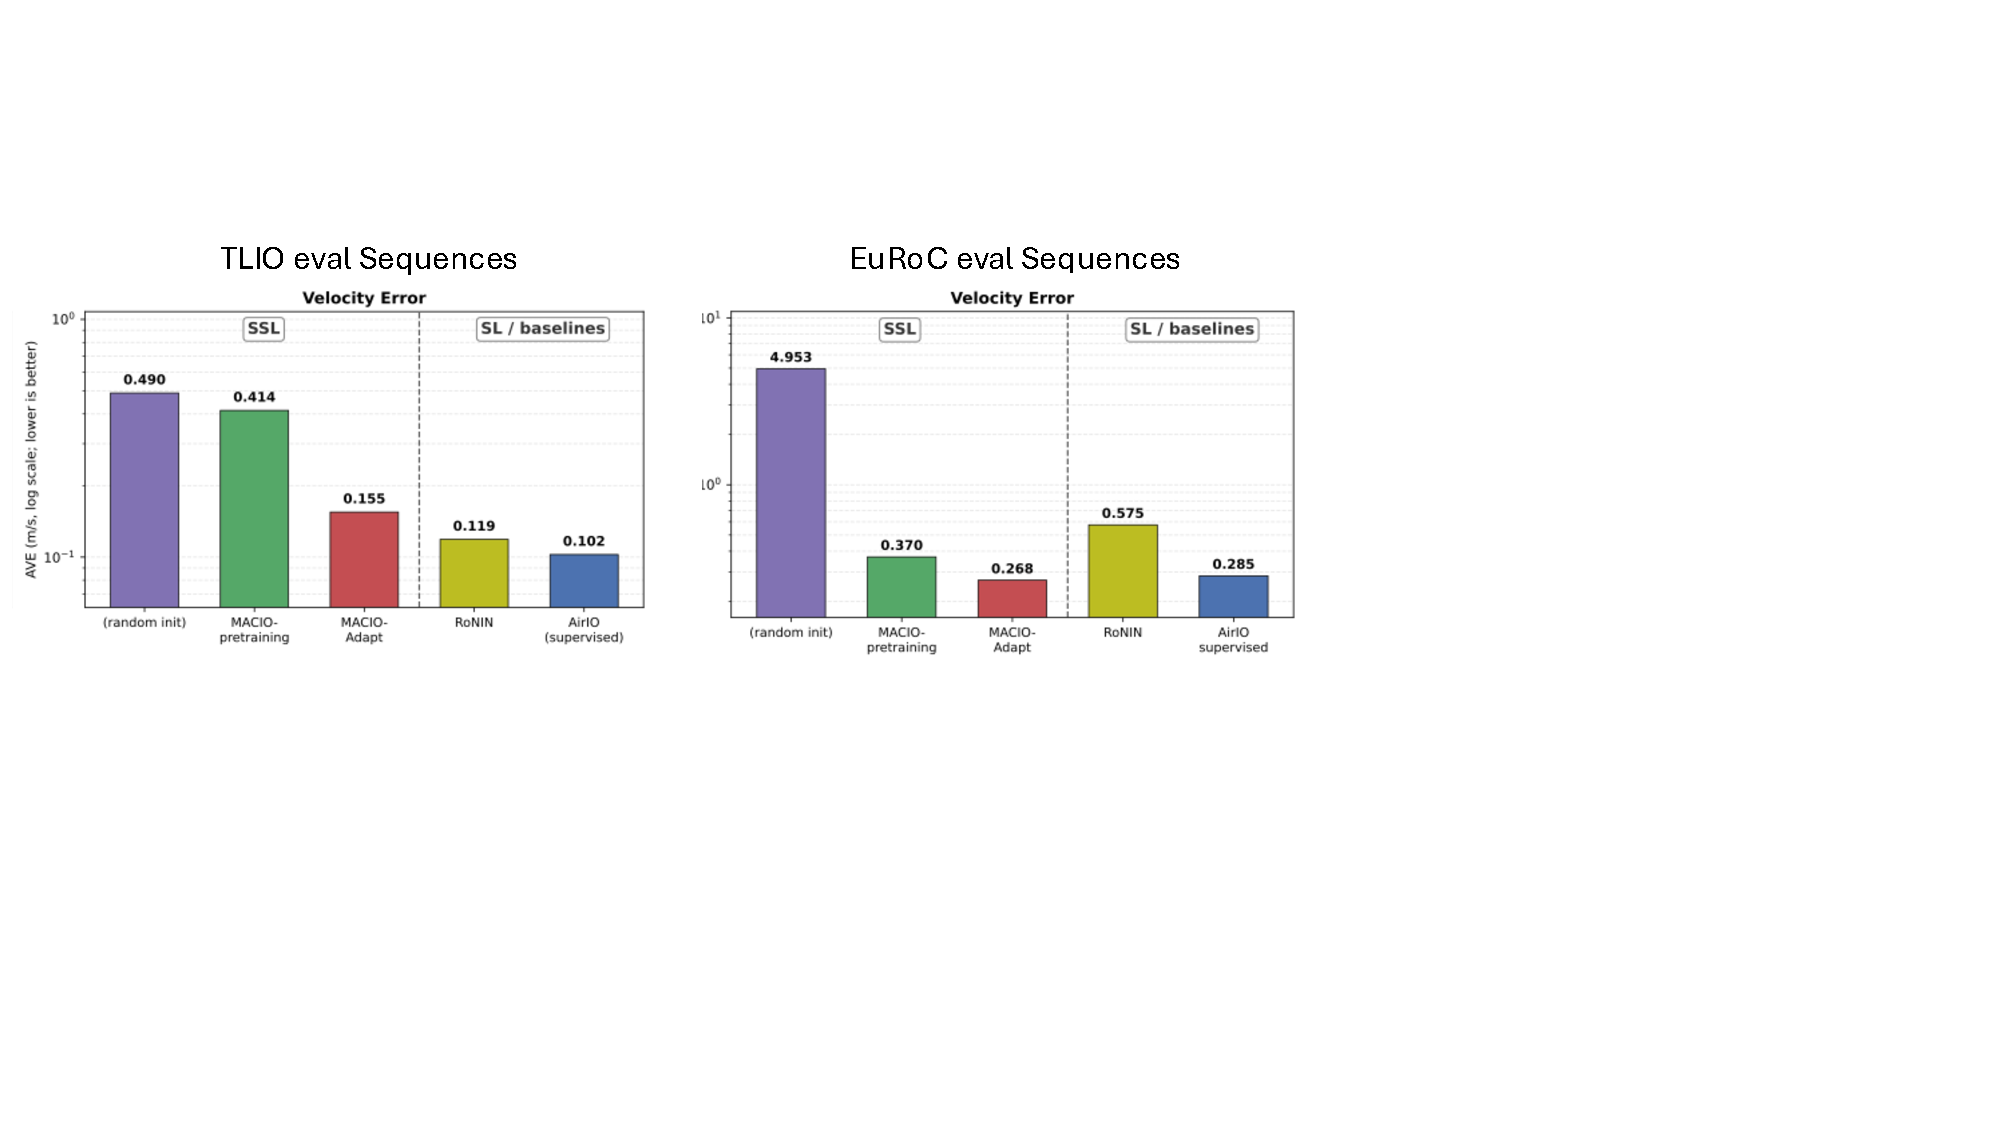
\includegraphics[width=\linewidth]{tex/ch6_macio/figs/setup1_ssl_results.pdf}
\caption[Setup 1 result: self-supervised MAC-IO improves velocity estimation from unlabeled IMU.]{\textbf{Setup~1 result: self-supervised MAC-IO improves velocity estimation from unlabeled IMU.}
Starting from random initialization, MAC-IO first learns local velocity increments from IMU preintegration and then distills the Step~2 PGO posterior into the motion network.
On TLIO and EuRoC evaluation sequences, the self-supervised result reduces AVE without using embodiment ground-truth labels during training.}
\label{fig:macio:setup1_ssl_results}
\end{figure}

On TLIO, MAC-IO Step~2 reduces AVE from $0.1025$~m/s (non-adapted reference) to $0.0398$~m/s, a $61.2\%$ reduction without any embodiment labels, matching the bars for the from-scratch protocol in \fref{fig:macio:setup1_ssl_results}; this final Step~2 value is the same number reported for the pretrained-model row of \tref{tab:macio:setup2_summary}, which we discuss separately in Setup~2.
The EuRoC pure self-supervised run improves AVE by 28.3\%, while its ATE remains worse than the adapted setting in Setup~2.
This split between local velocity accuracy and long-horizon position accuracy is consistent with the observability argument in \sref{sec:macio:method}.
Velocity-increment pretraining cannot identify a constant velocity offset, so a small residual offset in the random-init network can integrate into a noticeable position drift even after PGO posterior adaptation reduces per-frame velocity error.
On TLIO, where pedestrian motion contains frequent direction changes, the sequence-level graph quickly removes this offset; on the more agile and shorter EuRoC sequences, the same offset is harder to identify in a single window.

The two MAC-IO steps also play complementary roles within Setup~1.
Step~1 alone follows short-horizon velocity changes but leaves low-frequency offsets and occasional discontinuities, because its Mahalanobis loss only constrains differences between velocities.
Step~2 then resolves the offset by fusing the same preintegration teacher with the Step~1 network's velocity factors and distilling the optimized posterior back into the network.
\fref{fig:macio:setup1_stage2_ssl_sequence} visualizes this distillation on a TLIO sequence: the Step~2 PGO target tracks the ground-truth body-frame velocity that the Step~1 network only loosely follows, and after distillation the same network reproduces the posterior trace without any pose or velocity label.
The same plot also indicates that the PGO posterior covariance, distilled through the unlabeled KL term in \eref{eq:macio:posterior_adaptation_loss}, contracts the network covariance head where the optimized graph is confident and widens it where the graph residual is large.
This calibration behavior is what later allows the adapted network to be safely fused with deployment-time filters in Setup~2.

\begin{figure}[!htbp]
\centering
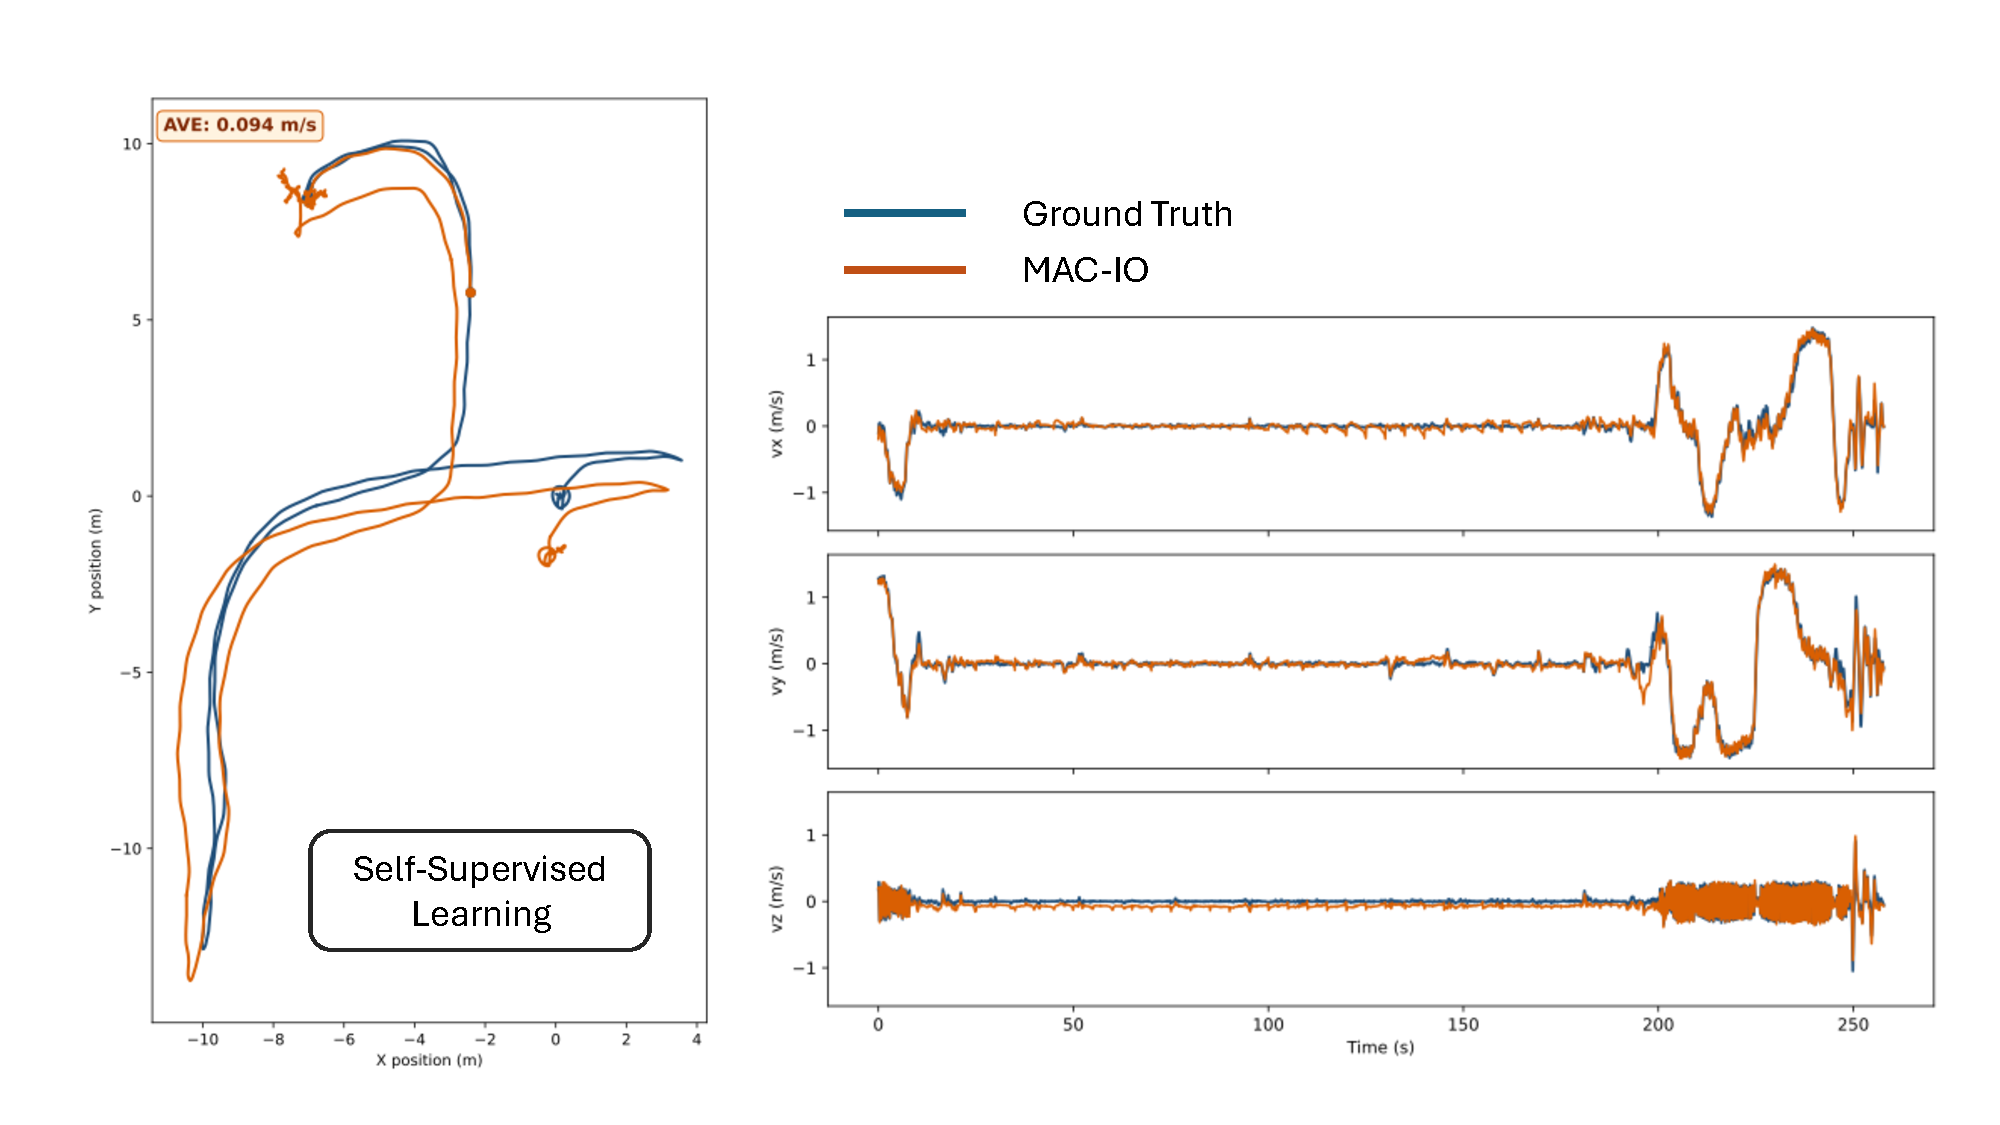
\includegraphics[width=0.78\linewidth]{tex/ch6_macio/figs/setup1_stage2_sequence.pdf}
\caption[Setup 1 result: MAC-IO learns from unlabeled IMU by distilling a Step 2 PGO posterior.]{\textbf{Setup~1 result: MAC-IO learns from unlabeled IMU by distilling a Step~2 PGO posterior.}
Starting from a network trained only with Step~1 velocity-increment self-supervision, MAC-IO builds a pose graph on the unlabeled training sequence, extracts posterior velocity and covariance pseudo-labels, and fine-tunes the same network without ground-truth labels.
Ground truth is shown only to evaluate and visualize the Setup~1 self-supervised result.}
\label{fig:macio:setup1_stage2_ssl_sequence}
\end{figure}

\subsection{Setup 2 Result: Pretrained-Model Adaptation}
\label{sec:macio:setup2_result}

Setup~2 evaluates MAC-IO as a deployment-time adaptation method.
The motion network is initialized from a supervised AirIO checkpoint trained on the labeled training split~\cite{qiu2025airio}, and MAC-IO then adapts it on unlabeled IMU using the PGO posterior teacher.
\tref{tab:macio:setup2_summary} reports each row as the multiplicative AVE and ATE reduction over the AirIO baseline so that improvements compose across the network, filter, and graph stages.

\begin{table}[!htbp]
\centering
\caption[Setup 2 results: adapting a pretrained IO model with unlabeled IMU.]{Setup~2 results: adapting a pretrained IO model with unlabeled IMU.
Each metric cell reports the multiplicative error reduction from AirIO (baseline) in parentheses, where larger is better and $1.0\times$ is the baseline.}
\label{tab:macio:setup2_summary}
\resizebox{\linewidth}{!}{
\begin{tabular}{lcccc}
\toprule
& \multicolumn{2}{c}{TLIO} & \multicolumn{2}{c}{EuRoC} \\
\cmidrule(lr){2-3}\cmidrule(lr){4-5}
Method & ATE $\downarrow$ & AVE $\downarrow$ & ATE $\downarrow$ & AVE $\downarrow$ \\
\midrule
RoNIN & 2.718 ($0.8\times\downarrow$) & 0.1187 ($0.9\times\downarrow$) & 5.276 ($0.6\times\downarrow$) & 0.575 ($0.5\times\downarrow$) \\
AirIO (baseline) & 2.187 ($1.0\times\downarrow$) & 0.1025 ($1.0\times\downarrow$) & 3.403 ($1.0\times\downarrow$) & 0.285 ($1.0\times\downarrow$) \\
MAC-IO Step~1 & 1.589 ($1.4\times\downarrow$) & 0.0858 ($1.2\times\downarrow$) & \textbf{2.807 ($1.2\times\downarrow$)} & 0.210 ($1.4\times\downarrow$) \\
MAC-IO Step~2 & 1.772 ($1.2\times\downarrow$) & 0.0398 ($2.6\times\downarrow$) & 3.163 ($1.1\times\downarrow$) & 0.184 ($1.5\times\downarrow$) \\
\midrule
TLIO (EKF) & 1.702 ($1.3\times\downarrow$) & 0.0921 ($1.1\times\downarrow$) & 10.427 ($0.3\times\downarrow$) & 1.646 ($0.2\times\downarrow$) \\
AirIO + EKF & 1.727 ($1.3\times\downarrow$) & 0.0785 ($1.3\times\downarrow$) & -- & -- \\
MAC-IO Step~2 + EKF & 1.705 ($1.3\times\downarrow$) & 0.0474 ($2.2\times\downarrow$) & 3.176 ($1.1\times\downarrow$) & 0.191 ($1.5\times\downarrow$) \\
\midrule
AirIO + PGO & 1.683 ($1.3\times\downarrow$) & 0.0398 ($2.6\times\downarrow$) & 2.810 ($1.2\times\downarrow$) & \textbf{0.1713 ($1.7\times\downarrow$)} \\
MAC-IO Step~2 + PGO & 1.788 ($1.2\times\downarrow$) & \textbf{0.0334 ($3.1\times\downarrow$)} & -- & -- \\
\bottomrule
\end{tabular}}
\end{table}


The two MAC-IO steps tighten the pretrained network at the network level before any deployment-time fusion.
On TLIO, Step~1 alone reduces AVE by $1.2\times$ and ATE by $1.4\times$ over the AirIO baseline, showing that velocity-increment pretraining still finds residual structure in unlabeled deployment IMU even when the network already saw labeled data.
Step~2 further improves AVE by $2.6\times$ on TLIO and $1.5\times$ on EuRoC, while ATE remains close to the baseline because raw integration is still dominated by accelerometer noise.
The improvement is largest where the supervised checkpoint had the most residual velocity error, which matches the role of the PGO posterior as a sequence-level corrector for the local network output.

Combining the adapted network with deployment-time filtering or graph optimization shows that the gains compound rather than overlap.
The TLIO EKF backbone, which is the primary deployment configuration in TLIO~\cite{liu2020tlio}, becomes noticeably more accurate when its velocity factor is supplied by the MAC-IO Step~2 network: AVE drops from $0.0921$~m/s under the TLIO EKF baseline to $0.0474$~m/s with MAC-IO Step~2 + EKF, a $2.2\times$ AVE reduction over AirIO.
At the graph level, MAC-IO Step~2 + PGO reaches $0.0334$~m/s AVE on TLIO, a $3.1\times$ reduction over AirIO and the strongest velocity result in the table.
On EuRoC, the same adapted network gives a $1.5\times$ AVE reduction with EKF and matches AirIO+PGO at the trajectory level while preserving the network-level $1.5\times$ AVE gain, indicating that the unlabeled posterior teacher does not undo the supervised motion prior on this dataset but sharpens it where the supervised checkpoint was already good.

These trends are consistent with the design of Setup~2.
The same factor graph that produced the Step~2 pseudo-labels also acts as the deployment-time estimator, so a network whose velocity and covariance head are aligned with that posterior provides a better-conditioned input both to a tightly coupled EKF and to an inference-time PGO.
Compared with external baselines such as RoNIN, which underperforms AirIO on both ATE and AVE, MAC-IO Step~2 improves over the supervised reference using only unlabeled IMU and the same teacher already used at deployment, supporting the use of PGO posterior adaptation as a label-free deployment-time refinement step.

\section{Conclusion and Discussion}
\label{sec:macio:conclusion}

This chapter presents MAC-IO, a self-supervised pretrain-then-adapt framework that learns inertial odometry on a new embodiment from unlabeled IMU.
The framework leverages the universal physical structure of IMU integration in two complementary steps.
Embodiment pretraining (Step~1) matches network velocity increments to a frozen AirIMU preintegration teacher under a Mahalanobis loss, learning short-horizon motion changes that transfer the embodiment-specific motion prior without requiring labels.
PGO posterior adaptation (Step~2) then resolves the constant velocity offset that Step~1 cannot observe by fusing the same teacher with the network's velocity factors in a sliding-window pose graph and distilling the resulting velocity and covariance posterior back into the network as dense pseudo-labels.
This separation makes the local and sequence-level roles of self-supervision explicit and lets the same posterior teacher both train the network and serve as the deployment-time estimator.

Experiments confirm that the two steps are complementary and that the framework supports two deployment modes.
In the from-scratch setting, the fully self-supervised protocol reaches the Step~2 AVE shown in \fref{fig:macio:setup1_ssl_results} on TLIO without any embodiment labels, a $61.2\%$ reduction over the non-adapted reference.
In the pretrained-model setting, the same PGO posterior adaptation improves a supervised AirIO checkpoint by the multiplicative reductions reported in \tref{tab:macio:setup2_summary}: $2.6\times$ in network AVE on TLIO and $3.1\times$ when combined with PGO at inference, while a $1.5\times$ AVE improvement on EuRoC shows that the unlabeled posterior teacher sharpens rather than undoes the supervised motion prior.
These results indicate that an unlabeled IMU stream, paired with a metrics-aware preintegration teacher, contains enough sequence-level information to retrain or refine an IO network for a new embodiment.

MAC-IO closes the inertial branch of this thesis by combining the differentiable preintegration and uncertainty model from AirIMU (Chapter~\ref{chapter:airimu}) with the body-frame motion network and EKF deployment from AirIO (Chapter~\ref{chapter:airio}) into a self-supervised adaptation loop.
The metrics-aware covariance that AirIMU exposes is what makes the Mahalanobis Step~1 loss and the IMU factor weights in Step~2 well calibrated, and the body-frame velocity head from AirIO is what the PGO posterior distills into.
Future work will extend the present TLIO and EuRoC evaluation to additional embodiments that span more challenging motion regimes, including aggressive racing flight on Blackbird and legged locomotion on a quadruped platform, and will report results per embodiment to test whether MAC-IO learns embodiment-specific priors rather than a single universal velocity prior.
A natural further step is to couple the adapted IO network with the visual-inertial initialization framework of Chapter~\ref{chapter:macinit}, so that label-free embodiment adaptation can also support robust bootstrap of full visual-inertial SLAM on new platforms.
